\leadchapter{
  This chapter is a general introduction to the Hawkes processes and the challenges explored in this manuscript.
  After a succinct presentation of the Hawkes processes with excitation, 
  we contextualise the state-of-the-art literature concerning estimation methods in Section~\ref{sec:chap0_introduction}. 
  This allows us to exhibit the two paradigms that are studied in this work: inhibtion and imperfect data. 
  A general outline of this manuscript is described in Section~\ref{sec:chap0_outline} along with the main questions that guided our research.
  Section~\ref{sec:chap0_inhibition} pertains to the parametric estimation of both univariate and multivariate Hawkes processes with eventual inhibiting interactions (Chapters~\ref{chapter:univariate_inhibition} and \ref{chapter:multivariate_inhibition}).
  Section~\ref{sec:chap0_missing_data} presents our contributions to the study of exciting Hawkes processes by accounting for certain models of imperfect data (Chapters~\ref{chapter:spectral_superposition} and \ref{chapter:spectral_thinning}).
}

\chapter{Introduction}

\section{Statistics for Hawkes processes: the mathematical setting}\label{sec:chap0_introduction}
    \subsection{At the origin: a self-exciting point process}
    %\textbf{Point processes.}
    In probability and statistics, the modelling of random collections of points in a certain space is commonly done through a point process.
    This particular version of stochastic processes is constructed around studying the spatial distribution of such indivisible elements.
    When studying point processes in the real line $\RR$ (or the half line $\RR_{\geq 0}$), the natural order of this space often incurs an ordering of any countable sequence of points $(T_k)_{k\in\ZZ}$: we talk then of \emph{temporal} point processes.

    In statistics, it is a common question to try and analyse the dynamics behind the occurrences of a certain phenomenon: the time of arrival of buses at a bus stop, the apparition of symptoms in a population or earthquake incidents in a region of the world.
    The simplest of models for point processes is the homogenenous Poisson process, where the waiting time between any two event times is distributed as an exponential random variable with a parameter $\lambda > 0$ known as the intensity of the process.
    A natural extension of this model is obtained by allowing the intensity to be a deterministic non-negative function $\lambda:\RR \to \RR_{\geq0}$, adding a temporal dependance to point arrivals.
    The more complex becomes the phenomena at the center of a study, the more intricate becomes the modelling of point processes as a result. 

    \textbf{The Hawkes process.}
    In 1971, Alan G. Hawkes introduced his model of self-exciting point processes \parencite{Hawkes1971}, which would come to be known later as the Hawkes point process.
    He defines this model through a past-dependant intensity function $\lambda:\RR\to\RR_{>0}$, that for any instant in time $t$, the intensity is expressed through the history $\mathcal{H}_t$ of process $N$ up to $t$, and was originally defined as:
    \begin{equation}\label{eq:chap0_univariate_linear_intensity}
        \lambda(t\mid \mathcal{H}_t) = \mu + \sum_{T_k \leq t}{h(t-T_k)}\,.
    \end{equation}

    \begin{remark}
      In the literature, it is common to omit writting the history $\mathcal{H}_t$ as it is directly implied that $\lambda$ has access to the entire past of the process.
      We follow this convention throughout this work, unless marked otherwise.
    \end{remark}

    The term $\mu$ is often referred to as the baseline intensity, which similar to the homogeneous Poisson process, dictates a constant rate of occurrences. 
    The dependance on the past is represented by the second term, where each event time that precedes $t$ contributes to the intensity function through the interaction function $h:\RR_{\geq0}\to\RR_{>0}$.

    It is mainly through this interaction function, also called kernel function, that the effects of the past are modelled. 
    The positivity of $h$ represents an excitation effect between points: each time an event $T_k$ occurs, it increases the value of the intensity function, increasing in turn the rate at which points appear.
    For stability reasons, $h$ is assumed to converge to $0$ as $t\to+\infty$, representing the dissipation of effects as time advances.

    Different shapes of $h$ allow to account for different effects. 
    On the one hand, strictly decreasing functions represent instantaneous effects such as the exponential \parencite{Ozaki1979, Ogata1988} or power-law kernels \parencite{Zhang2016}, which appear as spikes in the conditional intensity function. 
    On the other hand, the Rayleigh or gamma kernels \parencite{Lesage2022} can be chosen to represent delayed effects, where the maximum of the function is not at the origin $t=0$. Figure~\ref{fig:chap0_two_kernel_examples} illustrates two Hawkes processes with two different kernels.
    The properties of the conditional intensity function are intrinsically connected to those of $h$, and so when working in parametric settings, the choice of the kernel is essential and come with their advantages and inconveniences.
    The choice of smooth functions is transcribed as smoothness between two consecutive event times whereas the choice of kernels with bounded supports allow to leverage results from renewal process theory.

    \begin{figure}[!ht]
        \centering
          \includegraphics[width=\textwidth]{images/chapter0/two_kernel_examples.pdf}
        \caption{Kernel functions (top) and respective conditional intensity (bottom) functions of a Hawkes process started at $t=0$ for exponential (left) and gamma (right) parametrisations.
        }
        \label{fig:chap0_two_kernel_examples}
      \end{figure}

    \textbf{Clustering and branching structures.}
    A direct consequence of the expression of the intensity function as in Equation~\eqref{eq:chap0_univariate_linear_intensity} is that the Hawkes process model can be interpreted as a Poisson cluster process \parencite{Hawkes1974}.
    The most practical way of defining a cluster point process is as from a generative point of view.
    We begin by generating a homogenenous Poisson process in the real line $\RR$ with parameter $\mu$: these points $T_k^c$ are often called ancestors, immigrants or cluster centers.
    Each center generates a inhomogeneous Poisson process with intensity function $h(\cdot - T_k^c)$, forming a family of children points, also called descendants.
    The iteration is repeated with each new point generating its own subprocess until no descendants are generated.
    In the end, the cluster process, which with these notations would be a Hawkes process, is formed by the union of both ancestors and descendants.
    What distinguishes a Hawkes process is the fact that the support of the function $h$ is a subset of $\RR_{\geq0}$, meaning that each occurrence influences solely the future of the process.

    % Add a table with common kernels

    Aside from being a cluster Poisson process, we may remark that the generation algorithm describes a dynamic similar to a Galton-Watson branching process (see \textcite{Watson1875} for the discrete time version and \textcite[Chapter III]{Harris02} for the generalised version).
    More precisely, the Hawkes process can be seen as a time-continuous branching process with immigration:
    let us assume we observe the arrival of an immigrant at a time $T_k^c$.
    This immigrant will generate a first generation of children forming the first generation of points, or branches.
    As before, each child becomes its own parent by generating a new set of branches.
    A tree is then formed by the union of each immigrant and all of its descendants, and then the Hawkes process is once again formed by the union of all trees.

    A visualisation of both structures is illustrated in Figure~\ref{fig:branching_and_cluster05} for a Hawkes process with exponential kernel. 
    These two properties are what made Hawkes processes so attractive in the literature.
    From a theoretical point of view, the many existing developments of branching theory allowed to quickly obtain results concerning existence, stability, stationarity and other descriptors of the process.
    A main example concerns the existence of a Hawkes process: in order for the point process to have a finite number of points inside any bounded set, a necessary and sufficient condition is:
    \[\int_{0}^{+\infty}{h(t)\dd t} < 1\,.\]
    From a numerical point of view, we already introduced a simulation algorithm as described by the cluster structure and methods of estimation from both fields could be adapted in order to study Hawkes processes.
    
    \begin{figure}[!ht]
        \centering
          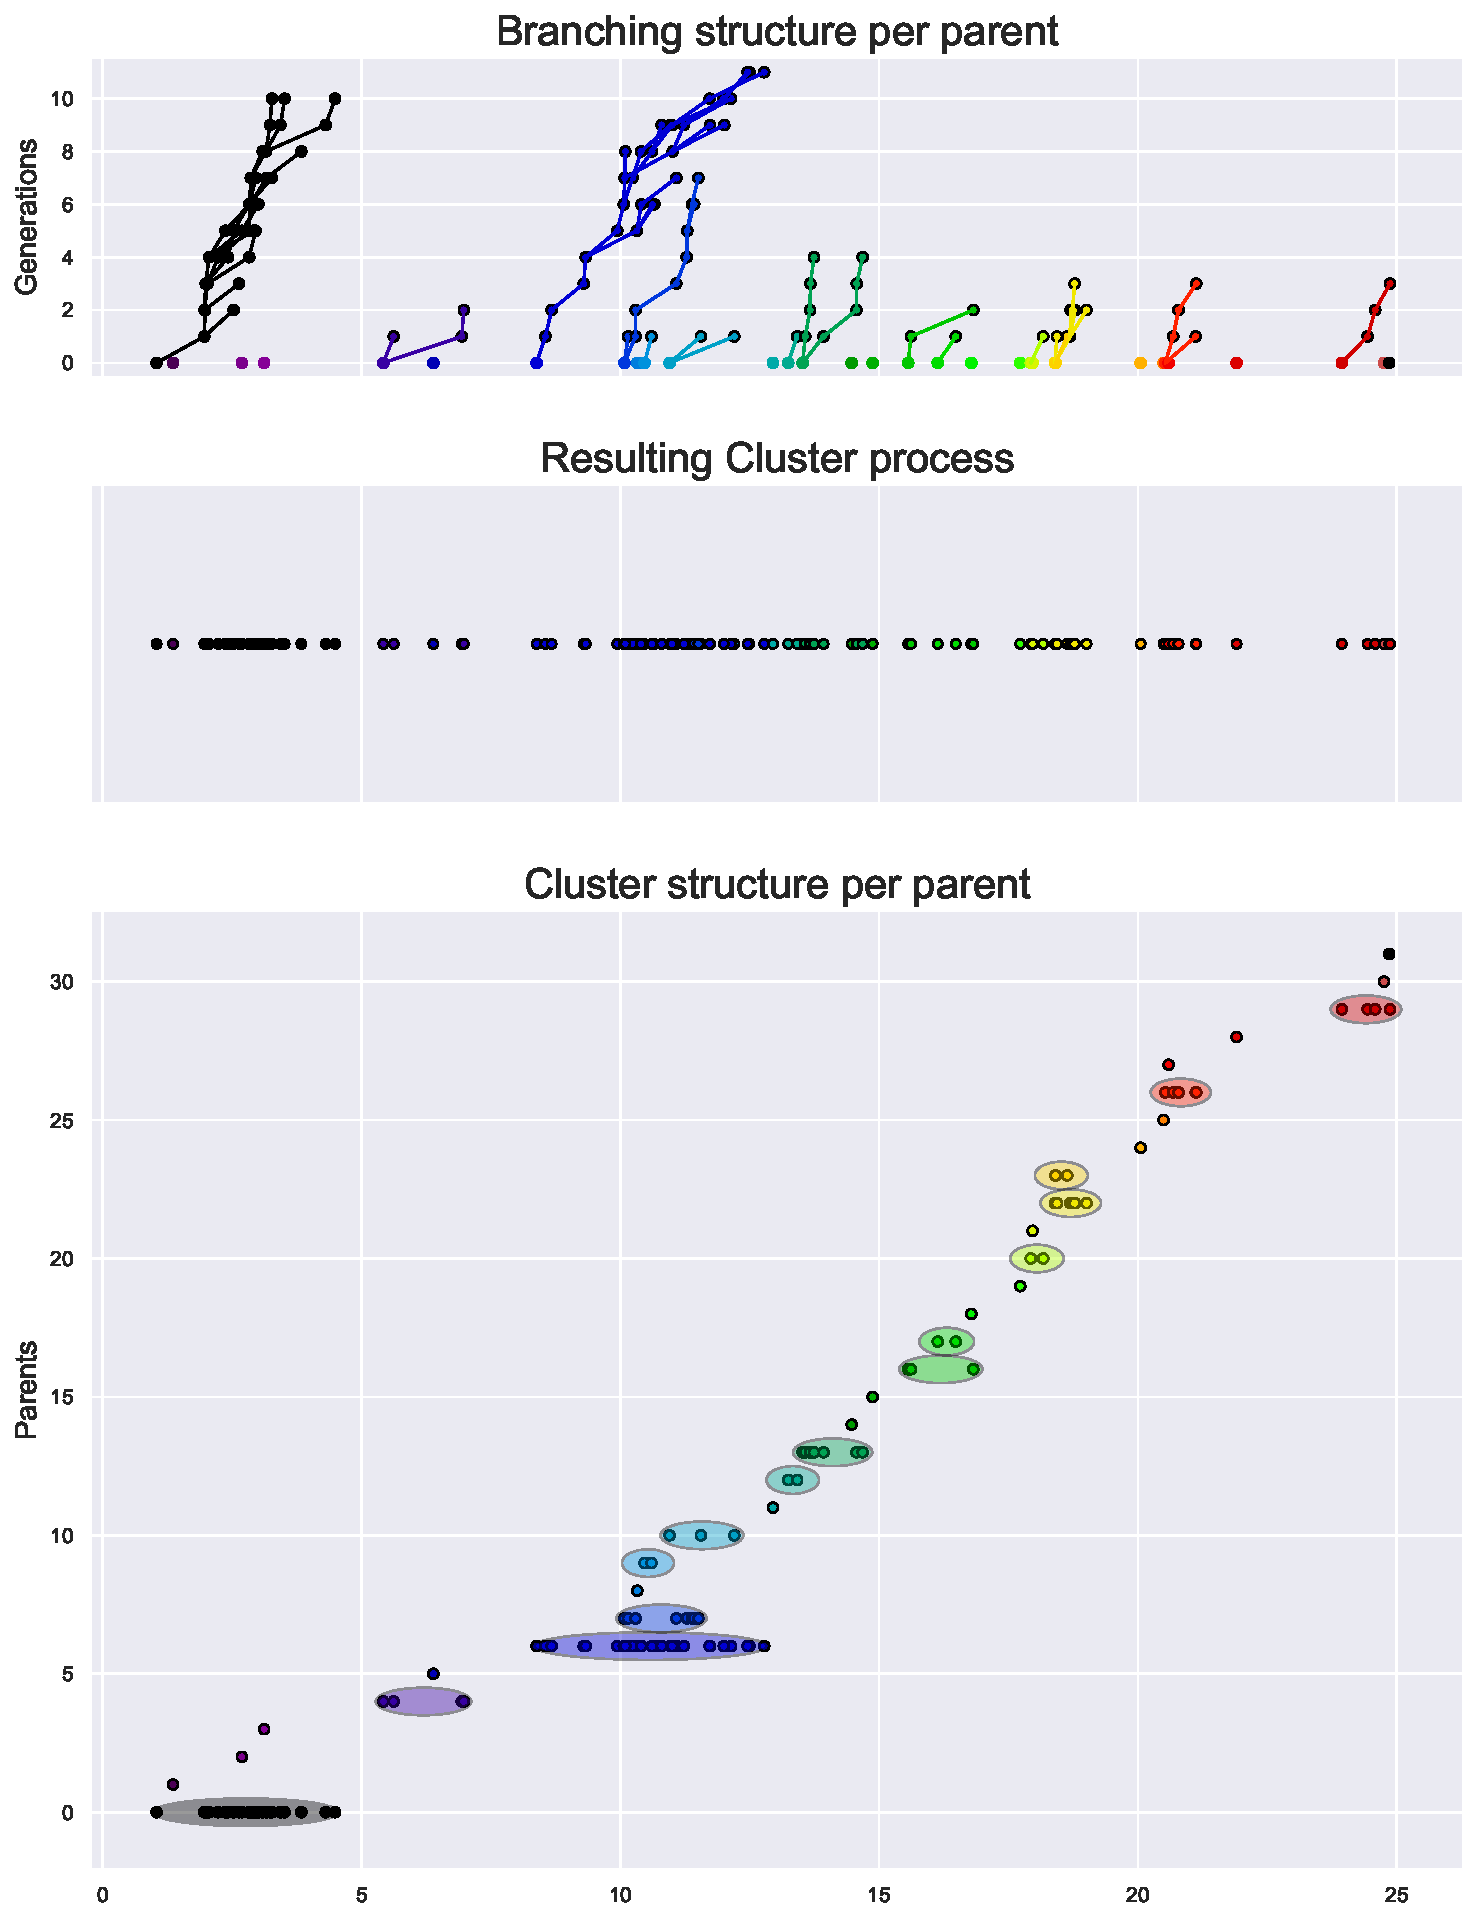
\includegraphics[width=0.95\textwidth]{images/chapter0/branching_and_cluster05.pdf}
        \caption{Illustration of both branching (top) and clustering (bottom) structures of an exponential Hawkes process (middle). Each color represents a single cluster/tree. Simulation is done through the cluster process algorithm.
        }
        \label{fig:branching_and_cluster05}
      \end{figure}

    It is these properties, and the quick developments that followed in the literature, that created a growing interest in other scientific fields.
    From this, different versions of the original self-exciting Hawkes process appeared in the literature, each one trying to accomodate more complex phenomena.

    \textbf{The multivariate Hawkes process.} Probably the most natural and useful was the definition of a \emph{multivariate} Hawkes process. 
    Instead of studying a single phenomenon (an univariate process), we define a $d$-variate Hawkes process as $d$ individual point processes $(N_i)_{i=1:d}$, 
    where each process is defined by a conditional intensity function $\lambda^i$:
    \[\lambda^i(t) = \mu_i + \sum_{j=1}^{d}\sum_{T_k^j \leq t}{h_{ij}(t-T_k^j)}\,, \qquad \text{for any $t\in\RR$.}\]

    In this formulation, each process $N^j$ has its own event times $(T_k^j)_{k\in\ZZ}$ and baseline intensity $\mu_i > 0$.
    What makes this model so interesting is the fact that it introduces interaction between processes, which is seen in the second term of the intensity.
    The kernel functions $h_{ij}$ represent the effect of points from $N^j$ on process $N^i$.
    This model allows to study a group of individuals linked by a network of interactions, adding a new dimension of study for such processes.

    From modelling infection spread all the way to the study of clusters of earthquakes, approaching the study of Hawkes processes from a statistical point of view quickly became a necessity.

    \subsection{Inference and applications}

    \textbf{Statistical estimation.}
    Presenting an exhausting bibliography on statistical estimation for Hawkes processes would represent a titanical task, 
    specially due to the numerous alternative models introduced since their introduction.
    Nonetheless, we propose here a general overview of the estimation panorama in the literature for self-exciting Hawkes processes.
    
    Statistical models for Hawkes processes with excitation focus around estimating both the baseline intenisty $\mu$ and the interation function $h$.
    In parametric settings, many kernel functions are traditionnally used (as some mentioned in the previous section),
    each one defined by a parameter $\gamma\in\RR^m$ for a certain integer $m$.

    %\Add theta and statistical model

    To our knowledge, the very first paper implementing an estimation procedure in a parametric framework is \textcite{Adamopoulos1976}.
    In his work, the author proposes a study of exponential kernels for both univariate and bivariate Hawkes processes through the spectral log-likelihood,
    closely related to time series theory.
    Let us take the time to remark that the exponential kernel is often chosen as a parametric interaction function because the univariate Hawkes process becomes a Markov process.
    This allows for many simplification when computing many quantities proper to the study of point process.
    as seen in the implementation of the maximum likelihood estimator (MLE) in \textcite{Ozaki1979}.
    The expression of the log-likelihood of a general point process, for an observation in $[0, T]$, is:
    \begin{equation}\label{eq:chap0_loglikelihood}
      \ell_T(\theta) = - \int_{0}^{T}{\lambda(u)\dd u} + \sum_{k=1}^{N(T)}{\log(\lambda(T_k))}\,,
    \end{equation}
    where $N(T)$ is the number of points in the observation window. 
    Other implementations of the MLE include \textcite{Ogata1988, Guo2018} and \textcite{Lewis2011} with a penalised version optimised by an EM algorithm.
    An alternative approach leveraging the branching structure is proposed in \textcite{Veen2008}.
    Other traditional methods in settings include least-squares minimisation \parencite{Reynaud2010, Eichler2016, Kirchner2017}, 
    method of moments \parencite{DaFonseca2013},
    via the solutions of Wiener-Hopf equation \parencite{Bacry2016},
    through approximation with autoregressive models \parencite{Kirchner2017},
    to name a few.
    
    All of these references concern frequentist approaches of statistics, 
    and so it is essential to mention that an equal effort has been made from a Bayesian point of view.
    \textcite{Rasmussen2013} proposes two procedures through log-likelihood estimation: 
    one through the classical intensity function and another similar to \textcite{Veen2008} with the branching structure.
    In \textcite{Lemonnier2014}, the authors propose an approximation through exponential kernels and taking advantage of the markovian properties.
    The multivariate case is deeply study in \textcite{Donnet2020} with illustrations on estimating the underlying interaction graph.
    
    This is a small insight on the plethora of approaches that have been developed in order to study these kind of processes.
    
    \textbf{Application fields.}
    The main motivation behind the works presented in this thesis, as it has been and continues to be for researches in this field,
    is to use the versatility of the model and its exceptional adaptability to propose new submodels.
    When confronted to real-world data, 
    researchers tend to reformulate and complexify the Hawkes model in order to better describe the studied phenomena. 
    
    The historical example is in seismology, 
    where the clustering structure becomes a way to study earthquakes and their replicas, as shown in \textcite{Adamopoulos1976,Ogata1988, Ogata1998} and more recent works \parencite{Kwon2023}.
    In this, the authors tend to add a spatial component to the model as this allows to incorporate spatial dependencies proper to seismic phenomena.
    %Further develop

    Including additional information in the model is a common approach, done often with marked version of the Hawkes process,
    which allows to incorporate addional covariates to the estimations. 
    In the study of social network interactions, as done in \textcite{Mishra2016,Rizoiu2017},
    by including information about each studied individual like number of followers or quality of the publications the authors improve the estimation of tweet cascades.

    Another approach is to render the baseline intensity a function of time, 
    as done in criminology \textcite{Lewis2011, Olinde2020}.
    This is particularly useful when working with data modelling daily behaviour, as different moments of a day imply different behaviour among individuals.

    Working in high dimensions allows to account for high number of individuals with sparse networks of interactions.
    Penalisation methods in the study of neuronal spike trains \parencite{Reynaud2013, Lambert2018}
    allow to reduce the support (non-null interactions) of the connectivity matrix.
    This allows to improve estimations, allow for better computational times and more importantly provide more explicative models for the experts.

    Many other fields include finance \parencite{Embrechts2011, Bacry2013, Lotz2024}, TV browsing analysis \parencite{Xu2016}, event data streams in football \parencite{Baouan2023, Narayanan2023}, 
    each one often accompanied with a new formulation of the Hawkes process.

    \subsection{Outline and challenges of this manuscript.}\label{sec:chap0_outline}

    Our goal in this thesis is to study two separate extensions of the Hawkes process model: the inhibition effect and the study of imperfect data.
    As a consequence, this manuscript is divided in two parts, with Chapter~\ref{chapter:background} presenting a succinct presentation of point processes theory, from a random measure approach, and the formalism of Hawkes processes.
    Let us note that all chapters are independent of each other and can be read as standalone documents.

    The first part of this thesis (Section~\ref{sec:chap0_inhibition}) concerns the study of the inhibition: 
    the opposite effect to excitation.

    \begin{itemize}
      \item Chapter~\ref{chapter:univariate_inhibition} presents a parametric estimation method for univariate Hawkes processes that accounts for both self-exciting or self-inhibiting interactions. 
      This is a joint work with Anna Bonnet and Maxime Sangnier. 

      The corresponding paper \parencite{bonnet2021} has been published in \textit{Statistics and Probability Letters}.
      
      Code is freely available at \url{https://github.com/migmtz/hawkes-inhibition-expon}

      \item Chapter~\ref{chapter:multivariate_inhibition} presents a parametric estimation method for multivariate exponential Hawkes processes with exciting and inhibiting interactions along with a model selection procedure. 
      This is a joint work with Anna Bonnet and Maxime Sangnier. 

      The corresponding paper \parencite{Bonnet2023} has been published in \textit{Statistics and Computing}.
      
      Code is freely available at \url{https://github.com/migmtz/multivariate-hawkes-inhibition}

    \end{itemize}

    The second part (Section~\ref{sec:chap0_missing_data}) consists in the study of imperfect observations of a Hawkes process realisation, similar to missing data formulations.

    \begin{itemize}
      \item Chapter~\ref{chapter:spectral_superposition} presents a parametric estimation method for exciting Hawkes processes whose event times are noised by those of a homogenenous point process, leveraging point process spectral theory. 
      This is a joint work with Anna Bonnet, Felix Cheysson and Maxime Sangnier. 

      The corresponding paper \parencite{Bonnet2024} has been submitted for publication.

      Code is available at \url{https://github.com/migmtz/noisy-hawkes-process}

      \item Chapter~\ref{chapter:spectral_thinning} presents the analysis of an inference method for thinned univariate Hawkes processes through spectral theory. 
      Additionally, it presents an improvement of $\ell_2$ penalisation through thinning subsampling for the spectral estimator.

      This chapter is an ongoing joint work with Felix Cheysson.
    \end{itemize}

    Although the models inbetween chapters may differ, our contribution follow a common thread by addressing the following four questions: 

    \begin{tcolorbox}
      \begin{itemize}
        \item What approaches can we take to establish parametric estimation procedures for more complex Hawkes processes dynamics?
        \item Under what conditions our statistical models are identifiable?
        \item How to evaluate and select the best estimators through data-driven methods?
        \item What modern statistical tools we can leverage to improve our inference procedures?
      \end{itemize}
    \end{tcolorbox}
    
    %These questions may serve as a general guide when reading this manuscript.

    %\subsection{Questions} %and contributions}
    % \begin{itemize}
    %     %\item In this thesis we study two extensions: 
    %     %\item In the first half (chapters) we study inhibition 
    %     %\item In the second half (chapters) we study missing data.
    %     \item Our studies are articulated along 3 general questions (i) what approaches for considering alternative or more complex dynamics than self-excitation in parametric and what properties can we establish; (ii) how to evaluate and select our models through data-based methods in multivariate cases (null interactions); (iii) what statistical tools allow us to improve inference.
    % \end{itemize}

% mentionner faire des outils accessible, partage du code (open source, facilité)
% mettre/valoriser les codes ici 
\section{Encouraging restraint: factoring in inhibition for Hawkes processes}\label{sec:chap0_inhibition}
    
    The original Hawkes process was proposed as a way of modelling the effect of excitation between points, which is characterised by the positivity of the interaction function $h$.
    Our first goal in this work is to study the opposite effect to this, which is commonly known in the literature as \emph{inhibition}.
    
    An inhibiting Hawkes processes consists on studying repulsion between points: each event will reduce the chances of others occurring for a certain period in time.
    Mathematically, a way of translating this effect is by allowing $h$ to take negative values. However, the non-negativity condition on $\lambda$ prevents us from take this approach without adding some constraints.

    One of the most common solutions is to define the \emph{non-linear} Hawkes process. In the univariate setting, let $h:\RR \to \RR$ and $\Phi:\RR\to\RR_{\geq 0}$ be two measurable functions. We define an univariate non-linear Hawkes process $N$ in the real half-line $\RR$ with event times $(T_k)_{k\in\NN}$ by the conditional intensity function, for any $t\in\RR$:
    \begin{equation}\label{eq:chap0_nonlinear_intensity}
      \lambda(t) = \Phi\left(\mu + \sum_{T_k \leq t}{h(t-T_k)}\right)\,.
    \end{equation}
    By allowing $h$ to be negative, the function $\Phi$ has to be a non-linear function. Existence of such processes is assured as long as $\Phi$ is an $L$-lipschitz function \parencite[Theorem 1]{Bremaud1996} such that:
    \[L\int_{0}^{+\infty}{h(t)\dd t} <1\,.\]
    Multiple choices exist in the literature like a clipped exponential function \parencite{Chornoboy1988,Carstensen2010,Gerhard2017},
    a softplus function \parencite{Mei2017},%s log(1+ exp(x/s))
    a sigmoid function \parencite{Menon2018}.
    
    In our work, we choose the positive part (ReLU) $\Phi(\cdot) = (\cdot)^+ = \max(0, \cdot)$ like in \textcite{Lemonnier2014, Hansen2015, Lu2018, Costa2020}.
    The intensity function (Equation~\eqref{eq:chap0_nonlinear_intensity}) becomes:
    \begin{equation}\label{eq:chap0_nonlinear_univariate_intensity}
      \lambda(t) = \left(\mu + \sum_{T_k \leq t}{h(t-T_k)}\right)^+\,,
    \end{equation}
    and the extension to a $d$-variate Hawkes process is:
    \begin{equation}\label{eq:chap0_nonlinear_multivariate_intensity}
      \lambda^i(t) = \left(\mu_i + \sum_{j=1}^{d}\sum_{T_k^j \leq t}{h(t-T_k^j)}\right)^+\,.
    \end{equation}

    % \begin{multicols}{2}
    %   [
    %   ]
    %   {\begin{center}\textbf{Univariate}
    %   \begin{equation}\label{eq:chap0_univariate_inhibition}
    %     \lambda(t) = \left(\mu + \sum_{T_k \leq t}{h(t-T_k)}\right)^+.
    %   \end{equation}\end{center}}
    %   {\begin{center}\textbf{Multivariate}
    %   \begin{equation}
    %     \lambda^i(t) = \left(\mu_i + \sum_{j=1}^{d}\sum_{T_k^j \leq t}{h_{ij}(t-T_k^j)}\right)^+.
    %   \end{equation}\end{center}}
    %   \end{multicols}

      %\begin{table}[!ht]
        % \begin{center}  
        %     \centering
        % \begin{tabular}{ c | c }
        %  \textbf{Univariate} & \textbf{Multivariate} \\
        %  $\displaystyle
        %   \lambda^i(t) = \left(\mu_i + \sum_{j=1}^{d}\sum_{T_k^j \leq t}{h_{ij}(t-T_k^j)^+}\right)\,.
        %   $ &
        % $\displaystyle
        % \lambda^i(t) = \left(\mu_i + \sum_{j=1}^{d}\sum_{T_k^j \leq t}{h_{ij}(t-T_k^j)^+}\right)\,.
        % $\\
        % \end{tabular}
        % \end{center}
      %\end{table}
    %\[\lambda^i(t) = \left(\mu_i + \sum_{j=1}^{d}\sum_{T_k^j \leq t}{h_{ij}(t-T_k^j)^+}\right)\,, \qquad \text{for any $t\in\RR$.}\]

    Our general contribution in the context of Hawkes processes with inhibition is to provide parametric estimation procedures in a frequentist framework through the maximum likelihood estimation.
    To our knowledge, and by the time of publication of both corresponding papers, other inference methods worked either in non-parametric \parencite{Reynaud2014,Bacry2016} or bayesian contexts \parencite{Rasmussen2013, Donnet2020, Sulem2021, Deutsch2022}.

    % \begin{itemize}
    %     \item Introduce the non-linear HP and give reference to other models of inhibition 
    %     \item Define inhibition in our case
    %     \item Bibliography of pre-existing methods (non parametric, bayesian).
    % \end{itemize}
    \subsection{Maximum Likelihood Estimation for Hawkes Processes with self-excitation or inhibition}
    
    In Chapter~\ref{chapter:univariate_inhibition}, we focus on the study of the univariate Hawkes process $N$ with intensity function described by Equation~\eqref{eq:chap0_nonlinear_univariate_intensity}.
    In order to establish the maximum likelihood estimator for a parametrised model of the intensity with parameter $\theta\in\Theta$, 
    it is necessary to obtain a closed-form expression of the log-likelihood:
    \[\ell_T(\theta) = - \int_{0}^{T}{\lambda_\theta(u)\dd u} + \sum_{k=1}^{N(T)}{\log(\lambda_\theta(T_k))}\,.\]
    %The integral in this term is commonly known as the compensator of $N$, noted:
    %\[\Lambda_\theta(T) = \int_{0}^{T}{\lambda_\theta(u)\dd u}\,.\]
    
    Our goal is to determine the values $t\geq 0$ such that $\lambda_\theta(t) > 0$ in order to exactly compute the compensator.
    For Hawkes processes with excitation, the linearity of the intensity function results in an explicit expression of $\ell$ without much trouble as shown in \textcite{Ozaki1979}.
    The main difficulty when including inhibition is that the cumulated effects from the past events may saturate process $N$, meaning that its intensity is null for a certain period in time.
    In the works of \textcite{Lemonnier2014}, the authors propose to approximate the computation in this context by ignoring the non-linear function.
    This allows them to circumvent this problem at the cost of assuming that the inhibition effects are small enough to be negligible.

    In order for us to obtain an exact computation of the loglikelihood that accounts for inhibition, we introduce two novel concepts: the \emph{underlying} intensity function $\lambda^\star$ and the \emph{restart times} $T_k^\star$.
    We define $\lambda^\star\colon \RR_{>0}\to \RR$, for any $t\leq 0$, as:
    \[\lambda^\star(t) = \mu + \sum_{T_k \leq t}{h(t-T_k)}\,,\]
    and the restart times $T_k^\star$ for any integer $k>0$ as:
    \[T_k^\star = \inf\{t\geq T_k \mid \lambda(t) > 0\}\,.\]

    The advantage of working with $\lambda^\star$ instead of $\lambda$ is that it inherits properties such as smoothness and strict monotony from the interaction function $h$ between any two consecutive event times $T_k$ and $T_{k+1}$.
    By assuming that $h$ is monotone and continuous, it follows that $T_k^\star$ is the moment from which both functions coincide.
    Our main contribution is establishing Proposition~\ref{prop:chap0_integral_cooldown}:

    \begin{proposition}\label{prop:chap0_integral_cooldown}
      For any $t>0$:
      
      \begin{equation}\label{eq:chap0_compensator_general}
      \int_{0}^{t}{\lambda(u)\dd u} =
      \begin{dcases}
          \mu t &\text{\qquad if $t<T_1$}\\
          \mu T_1 + \sum_{k=1}^{{N(t)-1}}{\int_{T_{k}^\star}^{T_{k+1}}{\lambda^\star(u)\,\mathrm{d}u}} + \int_{T_{N(t)}^\star}^{t}{\lambda^\star(u)\,\mathrm{d}u} &\text{\qquad if $t\geq T_1$}\,,
      \end{dcases}
      \end{equation}
      with the conventions that the sum is equal to $0$ if ${N(t)} = 1$ and the last integral is equal to $0$ if $t < T_{N(t)}^*$.
      \end{proposition}
    
    With this result, it suffices to obtain a closed-form expression of the restart times, which we explicit in the case of the exponential kernel function.
    We define then the maximum likelihood estimation procedure through an iterative algorithm to compute $\ell_T$.
    An outstanding property of our approach is that it allows to account for both self-exciting and self-inhibiting effects, without increasing the computational complexity.

    Our numerical study illustrates the efficiency of our estimator in multiple scenarios.
    As expected, we demonstrate the importance of correctly accounting for inhibition in our estimation procedure when compared to the approximation framework in \textcite{Lemonnier2014}, 
    Our approach provides satisfying estimates in the exponential context, specially when the inhibition effects are consequential.
    Finally, as a consequence of Proposition~\ref{prop:chap0_integral_cooldown}, we are able to implement a goodness-of-fit assessment of our models through the Time Change theorem of point processes \parencite[Theorem 7.4.IV]{DaleyV1}.
    This allows to introduce a hypthesis testing procedure that allows to evaluate the quality of our estimations on an independent set of observations.





    \subsection{Inference of multivariate exponential Hawkes processes with inhibition and application to neuronal activity}
    Chapter~\ref{chapter:multivariate_inhibition} builds on the bases established in the previous section by adapting our estimation procedure to multivariate Hawkes processes $N = (N^1, \ldots, N^d)$.
    Similarly to the univariate case, we propose to study the underlying intensity functions $\lambda^{i\star}$:
    \[\lambda^{i\star}(t) = \mu_i + \sum_{j=1}^{d}\sum_{T_k^j \leq t}{h_{ij}(t-T_k^j)}\,,\]
    but this time the monotony condition of $h_{ij}$ is not enough to retrieve useful properties on this functions.

    This is a consequence of the increased complexity concerning the dynamics of each subprocess of allowing both exciting and inhibiting effects to exist simultaneously.
    In the multivariate setting, it is possible for a subprocess $N^i$ to be saturated at an instant $t$ ($\lambda(t)=0$) and receive an external excitation of another subprocess.
    So, in order to simplify our problem, we restrict our study to the exponential kernel case $h_ij(t) = \alpha_{ij}\mathrm{e}^{-\beta_{ij} t}$ with the following mild assumption:

    \begin{assumption}\label{assu:chap0_beta}
      For each $i\in\{1,\ldots, d\}$, there exists $\beta_i\in\RR_+^*$ such that $\beta_{ij} = \beta_i$ for all $j\in\{1,\ldots, d\}$.
    \end{assumption}
    This allow us to recover the strict monotony of $\lambda^{i\star}$ between any two event times $T_{(k)}$ and $T_{(k+1)}$ of the general process $N$.
    With this, we adapt the expression of the restart times $(T_{(k)}^{i\star})_{k\geq 1}$, for each process $N^i$ and every event time $T_{(k)}$ allowing us to establish our first main contribution in the form of Lemma~\ref{lemma:chap0_restart_times}:

    \begin{lemma}\label{lemma:chap0_restart_times}
      If Assumption~\ref{assu:chap0_beta} is granted, then for each $i\in\{1,\ldots, d\}$ and any $k\geq1$: 
  
      \begin{equation}\label{eq:chap0_restart_times_exponential}
          T\park^{i\star} = \min{\adaptedpar{t^\star_k, T\park[k+1]}}\,.
      \end{equation}
      where
      \[t^\star_k = \adaptedpar{T\park + \beta_i^{-1}\log{\adaptedpar{\frac{\mu_i - \lambda^{i\star}(T\park)}{\mu_i}}}\II_{\{\lambda^{i\star}(T\park) < 0\}}}\]
  
      Furthermore,
      for all \(t \in (T\park, T\park[k+1])\),
      \[
        \lambda^i(t) =
        \begin{cases}
          \lambda^{i\star}(t) > 0 & \text{if } t \in (T\park^{i\star}, T\park[k+1])\\
          0 & \text{otherwise}.
        \end{cases}
      \]
      \end{lemma}

      With this result, we establish an exact procedure to compute the log-likelihood $\ell_T^i$ of each process $N^i$, giving us access to the complete log-likelihood $\ell_T$ and in turn, access to the maximum likelihood estimation method.
      
      Another complication brought upon by the multivariate setting is that the identifiability of our statistical model for the exponential Hawkes process is not as evident as in the univariate case.
      To partially answer this question, we provide an observational sufficient condition that allows to ensure an identifiable model, which ensures that our estimation procedure can be correctly implemented.
      Overall, this condition allows to avoid pathological situations either where some process $N^i$ is not observed (strong external inhibition effects), or there is a cyclical observation of points (strong internal inhibition effects).

      Our third contribution in this chapter is to provide a solution to the estimation of the interaction network of a multivariate Hawkes process.
      As it is common in real-data contexts, it is often unrealistic to assume that all functions $h_{ij}$ are non-null, meaning that all processes interacts with each other.
      For this, we introduce three different data-driven techniques based on a thresholding approach inspired by principal component analysis, and based on the construction of confidence intervals (student and empirical).

      Finally, we provide some insights on the performance of our procedures in both simulated and real-world contexts.
      The results for the simulated samples show a significant improvement with respect to other state-of-the-art methods \parencite{Lemonnier2014, Bacry2020}.
      In particular, when the interaction matrix $(\alpha_{ij})_{i,j=1:d}$ contains null entries, we implement our post-hoc procedures to obtain an estimation of the connectivity network before re-estimating all non-null entries on a reduced model.
      This provides the best estimations among all considered models.
      
      In the context of real data, we study ten samples of neuronal activity between 223 neurons of a red-eared turtle.
      This dataset represents a difficult task for any kind of estimation method. In order to improve our estimators we resort to a resampling technique proposed in \textcite{Reynaud2014}.
      Furthemore, we implement as in the univariate case a goodness-of-fit procedure accessed once again via the time change theorem.
      This is an important step in order to compare the quality of all models as we have no prior information on the real interaction network.
      To account for the high dimensionality, we incorporate a multiple testing procedure, which establishes our estimation through empirical confidence intervals as the best fitting model.

    % By allowing the interaction function $h$ to take negative values,
    % the occurrence of a point \emph{decreases} the rate of incoming event times.
    % The main difficulty of this approach originates from the non-negativity requirement on the conditional intensity function.
    % This is often controlled by introducing the concept of \emph{non-linear} Hawkes processes.



\section{Something is amiss: spectral methods for imperfect data}\label{sec:chap0_missing_data}
    
  In the second part of the thesis, we turn the spotlight to a common issue in statistics: 
  establishing efficient estimation procedures when the observed data is noised in some sense.

  In the context of point processes, a natural approach to define noised models is through the operations of thinning, superposition and jittering.
  These are mathematical transformations that allow to obtain new point processes through three different mechanisms:
  \begin{enumerate}
    \item The \textbf{superposition} of two point processes $X$ and $Y$, usually noted $X+Y$ is the point process defined by the ordered union of event times $T_k^X$ and $T_k^Y$.
    \item The \textbf{thinning} of a point process corresponds to erasing event times $T_k^X$ of a point process $X$ through a random rule.
    When point are erased independently from each other with a common probability $1-p$, we talk about a $p$-thinning of process $X$.
    \item \textbf{Jittering} a point process consists in the random displacement of points through the means of a probability distribution.
  \end{enumerate}

  The main interest of studying such alterations is to account for various measurement errors in real-world data. 
  The most commonly studied in the literature is jittering which tends to appear when spatial imprecisions add a layer of uncertainty, as in \parencite{Bonnet2022}. 
  Literature tends to focus on Poisson processes \parencite{Antoniadis2006, Hohage2016},
  with Hawkes processes being studied in \parencite{Trouleau2019, Deutsch2020}.

  Thinning is often used to represent missing data but has been scarcely studied in the literature. \textcite{Mei2019} propose a method to complete a sequence of times that are missing points via an LSTM model based on the Hawkes process.
  
  The study of superposition allows to account for observations that are contaminated by points originated by an external process, but are indistinguishable from those of the original process. 
  To our knowledge, the only work who studies this kind of noise is \textcite{Lund2000}, which in fact studies a general point process that is potentially noised by the three aforementioned mechanisms.
  Their work proposes an approach by defining a conditional log-likelihood, dependant on the original unnoised process, and approximate the maximiser through an iterative procedure studying "neighbouring" parameters, with an application to Hawkes processes.

  Other imperfect data models have been presented in \textcite{Linderman2014} in the form of missing marks, intervals or entire processes, where the authors favour a Bayesian approach through latent variables. 
  The last work we cite here is the work of \textcite{Cheysson2022} where the exact position of the points of a Hawkes process are not known. 
  Instead, the only information available is the number of points that fall inside equally-sized intervals.
  They leverage then the spectral theory of point processes and time series in order to provide an estimation procedure that does not necessitate the precise location of event times.
  
  Our contribution is to make use of the spectral theory of point processes, centered around the Bartlett spectrum \parencite{Bartlett1964} and the Whittle estimator \parencite{Whittle1952}, in order to study noised versions of the Hawkes process through superposition (Chapter~\ref{chapter:spectral_superposition}) and thinning (Chapter~\ref{chapter:spectral_thinning}).
  Another addition is to leverage the obtained inference method to incorporate a subsampling paradigm through thinning for small observation windows.
  The existing spectral theory for Hawkes processes is limited to exciting interactions, so we restrain our models to this framework.
  
  
    %\begin{itemize}
    %    \item Introduce the point process operations and provide missing data formalism. 
    %    \item Bibliography
    %\end{itemize}




    \subsection{Spectral analysis for the inference of noisy Hawkes processes}
    Chapter~\ref{chapter:spectral_superposition} is consacrated to the study of the superposition of a Hawkes process $H$ with exciting kernel functions and an independent homogeneous Poisson process $P$ with intensity $\lambda_0 > 0$.
    We consider the superposition of both processes, that we note $N$,
    and we assume that we have no prior knowledge on the origin of each event time $T_k^N$ (either Hawkes or Poisson).
    The intensity function of this resulting process is intractable and so any method based around it is innaccessible as a consequence. 
    
    As mentioned previously, we take inspiration from \textcite{Cheysson2022} in order to leverage the spectral approach of point processes to circumvent this issue. 
    The Bartlett spectrum $\Gamma^N$ of $N$ is a measure defined by the means of the Fourier transform of its reduced covariance measure.
    When this measure is absolutely continuous, its density is noted $f^N$ and often called the spectral density of the process.
    We can establish an estimation procedure of a parametric model for $f^N$ with parameter $\theta\in\Theta$ through the periodogram funciton $I^T$.
    For an observation $(T_k^N)_{k\geq 1}$ in $[0,T]$, the periodogram is defined, for any $\omega\in\RR$, as:
    \begin{equation}\label{eq:chap0_periodogram}
      I^T(\omega) = \frac{1}{T}\sum_{k=1}^{N(T)}\sum_{l=1}^{N(T)}{\mathrm{e}^{-2\pi \iu \omega (T_k^N - T_l^N)}}\,.
    \end{equation}
    Asymptotically, this quantity follows an exponential distribution of mean $f(omega)$ and so it is possible to define the maximum spectral log-likelihood estimator $\hat \theta$ as:
    \begin{equation}\label{eq:chap0_spectral_estimator}
      \hat \theta = {\arg\max}_{\theta\in\Theta} \left(-\frac{1}{T}\sum_{k=1}^{M}{\left(\log\left(f_\theta^N(\omega_k)\right) + \frac{I^T(\omega_k)}{f_\theta^N(\omega_k)}\right)}\right)\,.
    \end{equation}
    What makes this quantity so useful in our context is that it can be exactly computed without any information source of event times $(T_k^N)_k$. 

    To correctly work with these tools, it is necessary to consider stationary point processes,
    whichm for the case of Hawkes processesm necessitates to consider processes in the entire real line $\RR$.
    The spectral density of a Hawkes process is known in the literature \parencite[Example 8.2(e)]{DaleyV1}.
    We then establish a first result showing that the spectral density of a superposition $N = H + P$ is the sum of their respective spectral densities.
    Combining these two results, we obtain the general form of the spectral density of our noisy Hawkes process and so we can establish an estimation procedure by maximisation of the spectral log-likelihood.
    
    Our main contribution in the univariate setting is to establish conditions for the identifiability of $f^N$ for different parametrisations of the kernel function $h$. 
    The first result concerns the classic exponential kernel. 
    We show that the model is identifiable if and only if one of the four parameters (three for the Hawkes process and one for the Poisson process) is fixed, even though the distribution of $N$ is uniquely determined without this constraint.
    This being the most commonly used interaction function, we studied the uniform kernel and show that it is indeed identifiable.

    In the multivariate case, all tools from spectral theory exist and results are easily extended concerning the estimation procedure.
    Our contributions concern specifically the bivariate exponential Hawkes process noised this time by a bivariate Poisson process with common parameter $\lambda_0$.
    We present condition on the interaction matrix $(\alpha_{ij})_{1 \leq i,j \leq 2}$ that characterise either the identifiability or non-identifiability of the corresponding statistical model.

    Our work is concluded by a numerical study in both the univariate and bivariate cases when identifiability conditions are verified.
    We show in both cases that our estimators perform particularly well, specially for high levels of interaction effects and as the observation horizon $T$ increases.
    Our final contribution is to propose an ad-hoc procedure in the bivariate case that allows to determine the support of the interaction matrix by considering the empirical 5$\%$ quantiles of a sample of estimations, which in turn enhances the performance of our methods.
    




    \subsection{A numerical exploration of thinned Hawkes processes through spectral theory}
    The last Chapter~\ref{chapter:spectral_thinning} turns to the analysis of the thinning operation for point processes.
    We assume that we observe a partial process $H_p$ issued from thinning an univariate Hawkes process with a probability $1-p$ of erasing each point $T_k$, for $k\in\ZZ$.
    As previously mentioned, any method based on the conditional intensity function is unavailable, so we turn to spectral theory.

    All the tools presented in the previous subsection can still be implemented here, in particular the expression of the periodogram (Equation~\eqref{eq:chap0_periodogram}) remains unchanged.
    As a consequence, it can still be exactly computed even though we do not observe all points of the original process.
    In order to implement an inference procedure as defined by Equation~\eqref{eq:chap0_spectral_estimator}, we need to obtain an expression of the $p$-thinned process $H_p$.
    This is obtained in Proposition~\ref{prop:chap0_spectral_thinning}:

    \begin{proposition}\label{prop:chap0_spectral_thinning}
      Let $H$ be a stationary point process admitting a spectral density function $f^H$ and let $m_1$ be its average intensity.
      For any $p\in(0,1)$, let $H_p$ be a $p$-thinning of $H$.
  
      Then, $H_p$ admits a spectral density function, denoted $f^{H_p}$, such that for any $\omega\in\RR$:
      \begin{equation}\label{eq:chap0_spectral_thinning}
          f^{H_p}(\omega) = p^2 f^H(\omega) + p(1-p)m_1\,.
      \end{equation}
  
  \end{proposition}
    This result is obtained by leveraging the spectral theory of marked point processes as presented in \textcite{Bremaud2005}.
    As done in the superposition scenario, 
    we focus our study on the exponential kernel and we prove once again that the derived statistical model is identifiable if and only if one parameter is fixed.
    
    We present numerical results under this condition by fixing the value of the thinning parameter $p$. 
    In particular, we show that our estimation method is robust with respect to the level of thinning, with remarkable results when enough event times are available for inference.
    This is particularly encouraging, as the thinning procedure can dilute the interactions between the original points from process $H$.
    
    Our last contribution in this work is to make use of the thinning operation as a subsampling procedure when a single observation of $H$ is available in a small window of time.
    The use of subsampling for point processes has been done previously in the literature \parencite{Moller2003, Cronie2024, Coeurjolly2024} in order to improve estimation procedures or to introduce cross-validation paradigms.
    In our case, we focus on enhancing the quality of our spectral estimations by combining an $\ell_2$ penalisation with an averaged estimator obtained by thinning the unique observation of $H$.
    We show that our proposed procedure provides in general the best estimations when compared to another subsampling procedure and displays a net improvement of the relative $\ell_2$ error by reducing the high bias observed for the non-penalised estimator.
    
    




%\section{The numerical contributions}

%entrer titre et outline